\chapter{Implementation} \label{implementation}

\bigskip \bigskip 

The implementation of a knowledge graph for industrial risk assessment provides a structured approach to risk management. Querying the model for a specific use case and specific implementation scenario can be beneficial for the workflow of present day risk assessment. Discussed below are a few of such scenarios which are divided into three categories according to the use cases they might serve:

\begin{enumerate}
    \item Access general information
    \item Implementation of the knowledge graph in risk assessment
    \item Specific use case
\end{enumerate}

\section{Access general information}
Querying the model allows users to retrieve specific information on the ISO 12100 safety standard in a structured manner, which is particularly beneficial for new engineers during risk assessment. To access general information, the model can be extremely beneficial for two important reasons:

\begin{enumerate}
    \item Easy access to information
    \item Time saving access to information
\end{enumerate}

Discussed below are a few use cases from the perspective of the benefits that a new engineer can enjoy while using the knowledge graph over traditional approach.

\subsection{Easy access to information}
The knowledge model contains a vast amount of information and expertise which can also be enriched. By querying the model, a new engineer can gain access to a wealth of knowledge from previous risk assessment. It can prove to be a consistent source of information to make informed decisions. The knowledge graph could help the engineer to take decisions relying on two consistent sources of information - the expert's knowledge and the safety standard. Let's start with a very basic example that the engineer wants to learn about a machine according to the ISO 12100 standard. The following relations gives the corresponding information about a machine.
\begin{itemize}
    \item hasPhaseOfMachineLifeCycle - Gives all the phases of a machine's lifecycle.
    \item safetyDependentOn - Gives information about dependency of safety features.
    \item hasPart - Components of a machine.
    \item hasFeature - Gives all the features in general a machine possess.
    \item hasState - The possible states of a machine.
\end{itemize}

The following screenshot shows the query page on Machine:

% \bigskip\bigskip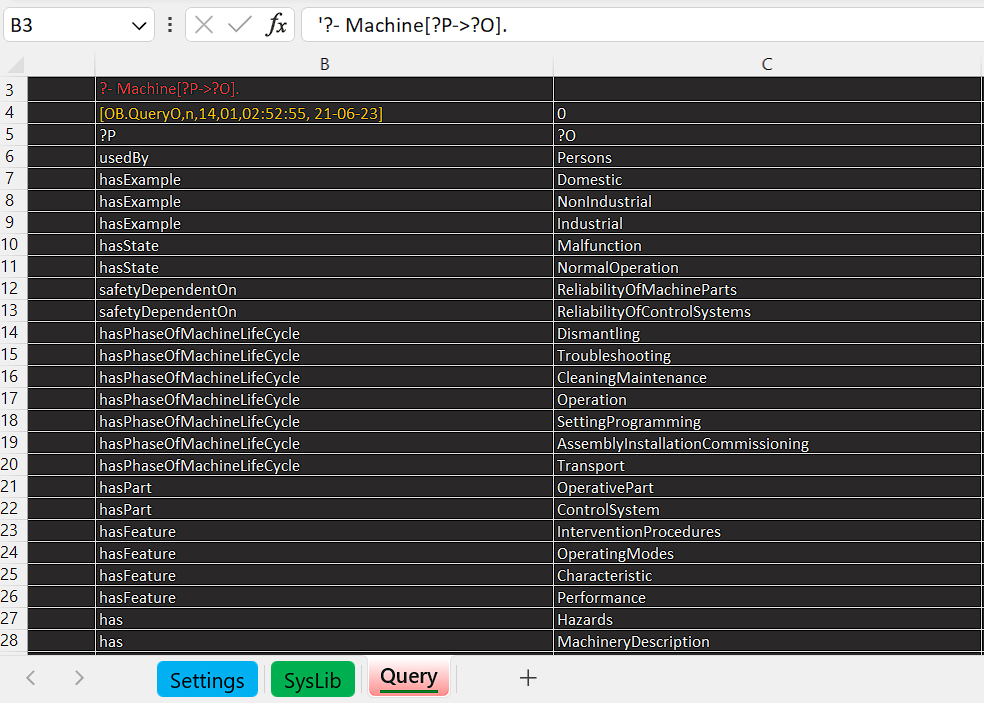
\includegraphics[width=\textwidth]{img/Machine.png}

\bigskip\bigskip \adjustimage{width=\textwidth, center, caption={Query on the concept Machine}, label={fig10}, nofloat=figure, vspace=\bigskipamount}{img/Machine.png}

\paragraph{} From the data it can be seen that one of the states of the machine could be Malfunction. A query on Malfunction can give more information as below:

% \bigskip\bigskip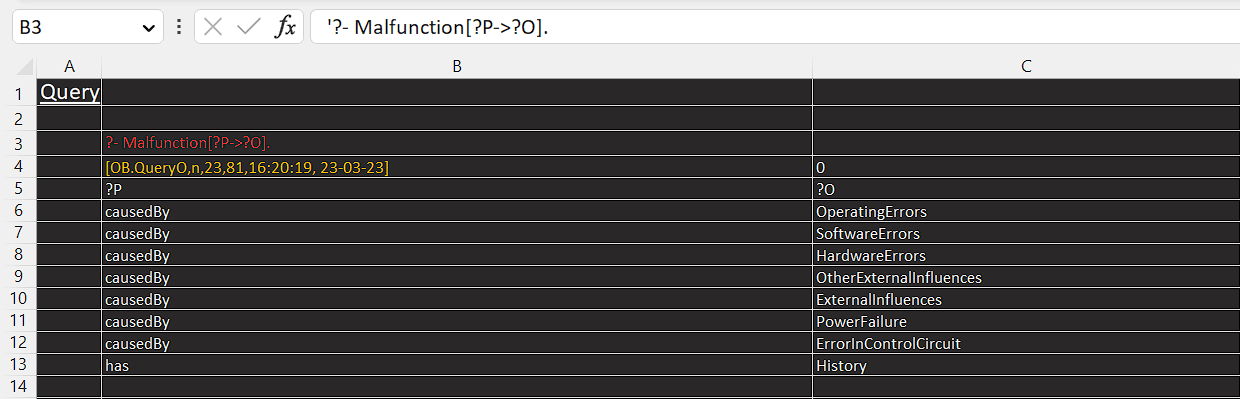
\includegraphics[width=\textwidth]{img/Malfunction.png}

\bigskip\bigskip \adjustimage{width=\textwidth, center, caption={Query on Machine state Malfunction}, label={fig11}, nofloat=figure, vspace=\bigskipamount}{img/Malfunction.png}

\bigskip\bigskip \adjustimage{width=\textwidth, center, caption={Graph visualisation of Machine state Malfunction}, label={fig11}, nofloat=figure, vspace=\bigskipamount}{img/malfunction_graph.png}

\paragraph{} It could be noted, that due to the connected nature of a knowledge graph, a Malfunction also shows up when there is a query for Hazards. Since a Malfunction is also a Hazard.

% \bigskip\bigskip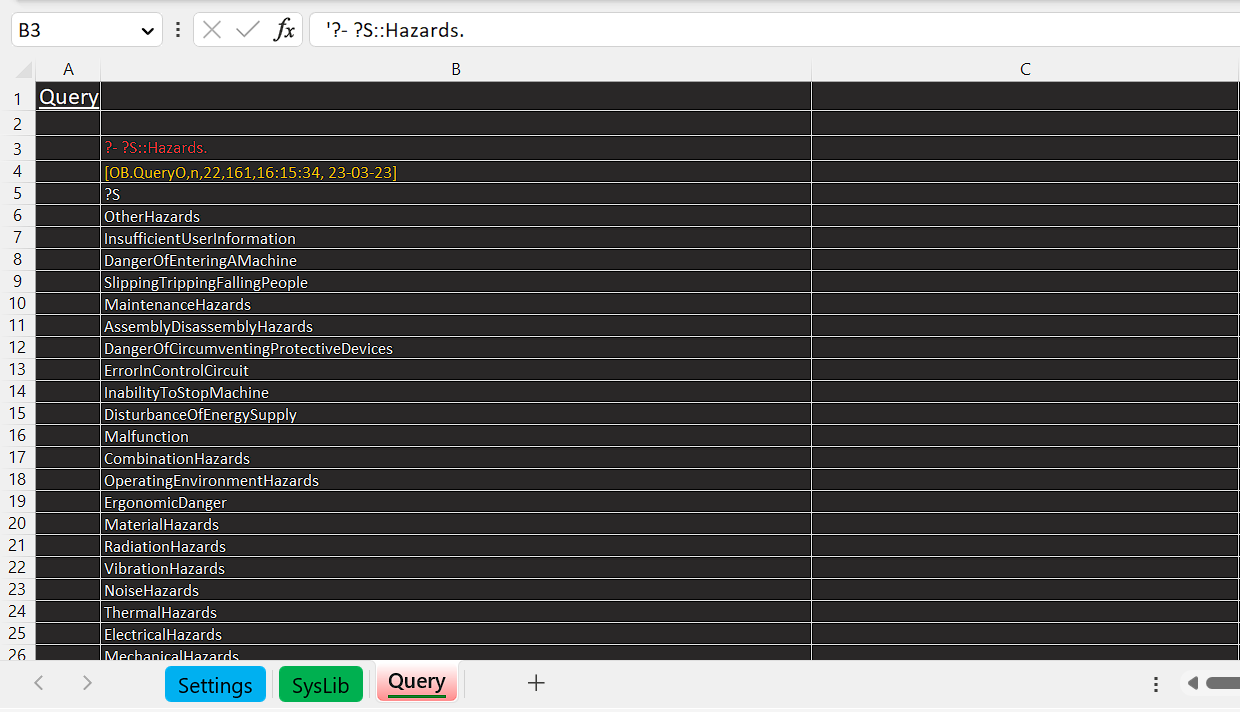
\includegraphics[width=\textwidth]{img/Hazards.png}

\bigskip\bigskip \adjustimage{width=\textwidth, center, caption={Query for the class Hazard}, label={fig12}, nofloat=figure, vspace=\bigskipamount}{img/Hazards.png}

\paragraph{} Another example can be taken here, for example a machine needs risk assessment. A simple query on RiskAssessment can give information about the three-step method (according to the ISO 12100) in a structured manner.

% \bigskip\bigskip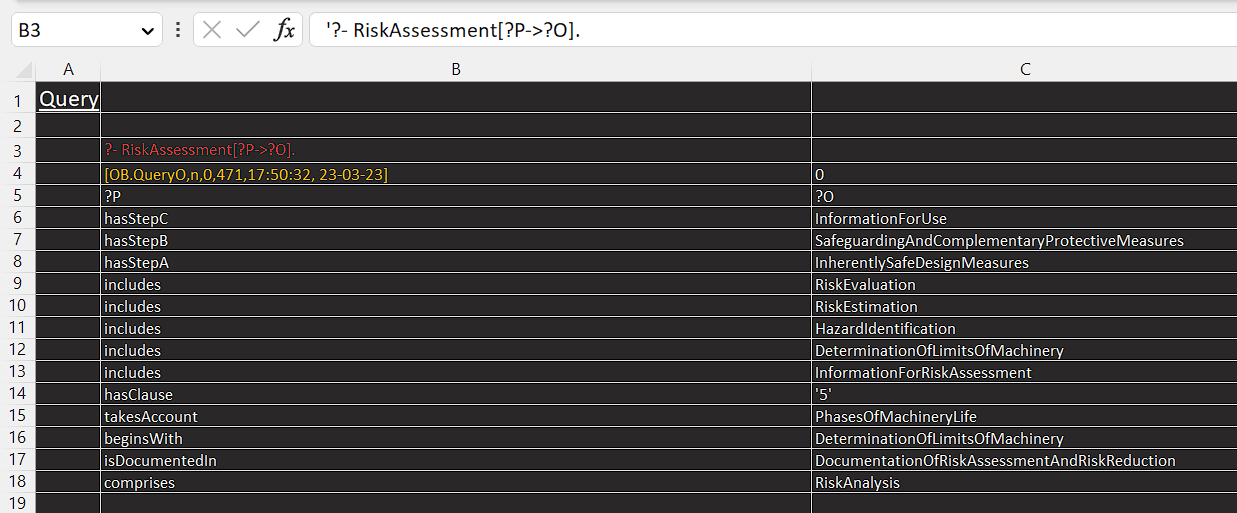
\includegraphics[width=\textwidth]{img/RiskAssessment.png}

\bigskip\bigskip \adjustimage{width=\textwidth, center, caption={Query on the concept RiskAssessment for a machine}, label={fig13}, nofloat=figure, vspace=\bigskipamount}{img/RiskAssessment.png}

\paragraph{} Each of the step here can be further queried for more information. One thing to note here, the hasClause relation shows the clause number to refer to the safety standard. For example a query on the third step, InformationForUse would give the following result:

% \bigskip\bigskip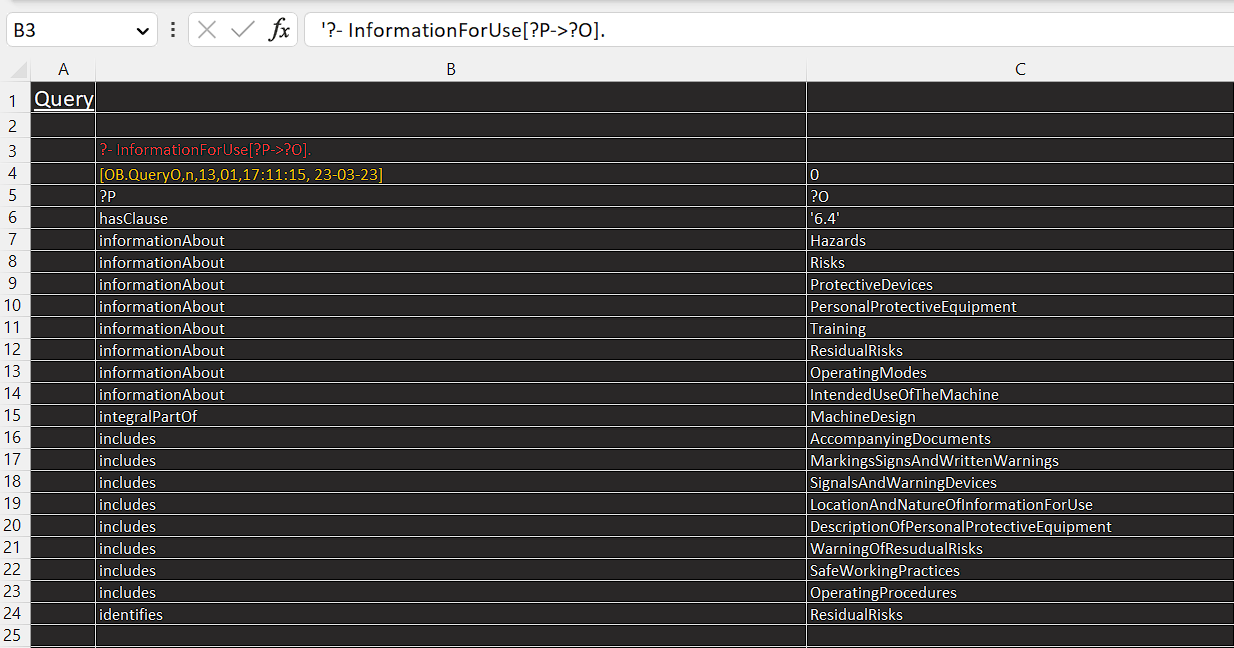
\includegraphics[width=\textwidth]{img/InformationForUse.png}

\bigskip\bigskip \adjustimage{width=\textwidth, center, caption={Query on the third step of risk assessment InformationForUse}, label={fig14}, nofloat=figure, vspace=\bigskipamount}{img/InformationForUse.png}

\paragraph{} Overall, the knowledge graph can be a useful tool for organizing and understanding complex information in a structured and intuitive way.

\subsection{Time-saving access to information}

\paragraph{} Querying a knowledge model can save a significant amount of time compared to conducting extensive research or seeking out advice from multiple experts. With the right query, a new engineer can quickly find relevant information and insights that can inform their decision-making process. It also cuts out the painstaking process of going through every line of a safety standard before every project of risk assessment. For example while working on a machinery, if the engineer wants to quickly learn about the Guards which comes under Inherently Safe Design Measures of the ISO 12100, can easily be done by querying the model. Otherwise, the engineer would have to go through the entire text written in the document to figure out each type of guard and their corresponding requirements which is an important data for risk assessment.

% \bigskip\bigskip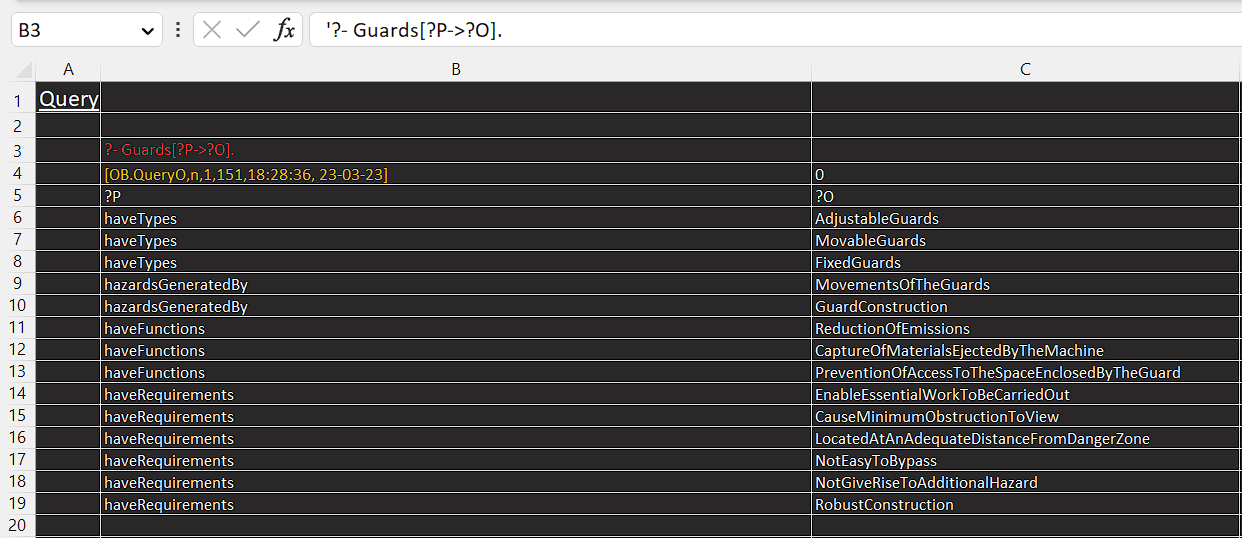
\includegraphics[width=\textwidth]{img/Guards.png}

\bigskip\bigskip \adjustimage{width=\textwidth, center, caption={Query on the concept Guards}, label={fig15}, nofloat=figure, vspace=\bigskipamount}{img/Guards.png}

The relations shown in the image are discussed below:

\begin{itemize}
    \item haveTypes - This relation gives all the types of the component.
    \item hazardsGeneratedBy - This relation gives the reason for the hazards.
    \item haveFunctions - This relation gives the functions of the component.
    \item haveRequirements - This relation gives the testing requirements of components according to ISO 12100.
\end{itemize}

The relations are pretty straightforward and from the query it is clear that there are three different types of guards. The functions of guards are displayed along with the cause of hazards from the guards. The general requirements for guards are also displayed. But if needed, specific requirements for a specific guard type can also be queried easily. For example, if the requirements for adjustable guards are needed, a quick query can give the data as below.

% \bigskip\bigskip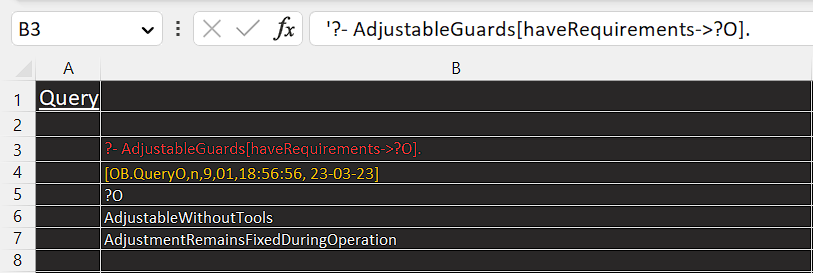
\includegraphics[width=\textwidth]{img/AdjustableGuards.png}

\bigskip\bigskip \adjustimage{width=\textwidth, center, caption={Query on the requirements for AdjustableGuards}, label={fig16}, nofloat=figure, vspace=\bigskipamount}{img/AdjustableGuards.png}

\paragraph{} A lot of other queries can be made which could be helpful in accessing general information from the knowledge graph.

\section{Implementation of the knowledge graph in risk assessment}
A knowledge graph can be a powerful tool that could be implemented in the current risk assessment process to identify and mitigate risks more effectively. This can be understood by a simple example. Suppose a new risk assessment on a Laser is to be performed. A query on the model can give information about the hazards that the laser may possess.

% \bigskip\bigskip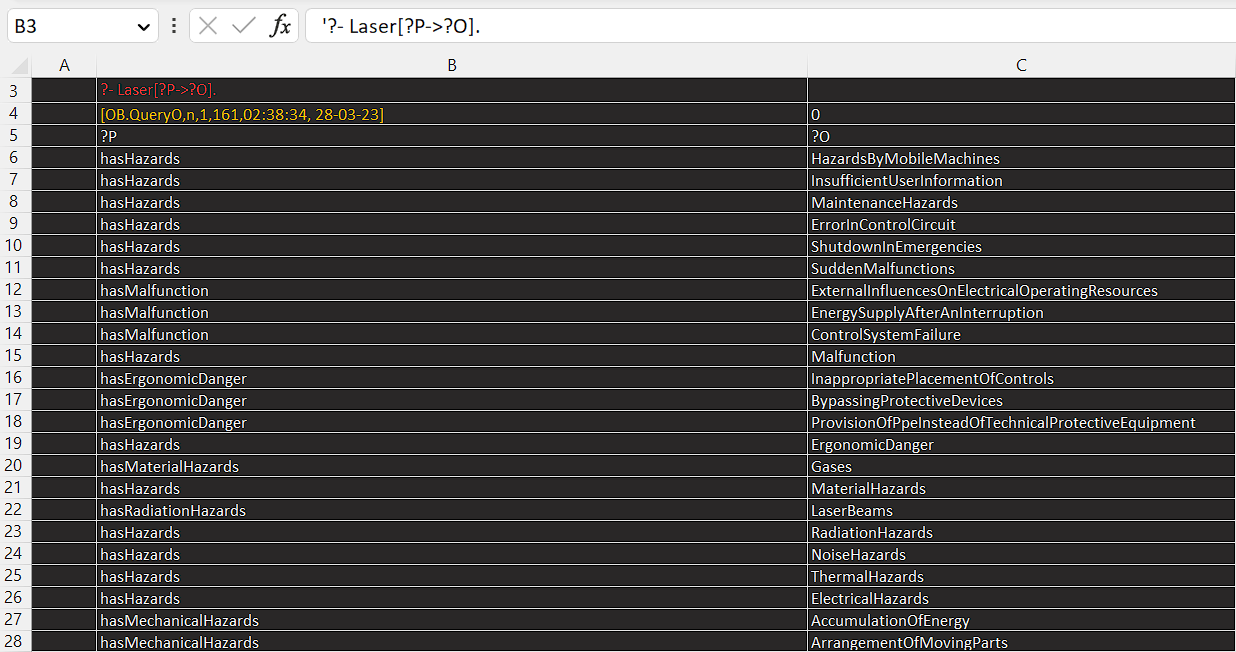
\includegraphics[width=\textwidth]{img/Laser.png}

\bigskip\bigskip \adjustimage{width=\textwidth, center, caption={Query on a machine Laser}, label={fig17}, nofloat=figure, vspace=\bigskipamount}{img/Laser.png}

Now that all the hazards of a laser are shown, it is required to mitigate the risks. For that more information is required for each hazard. Selecting one hazard at a time, for example, going with the Noise Hazard, query on the model can give the following information.

% \bigskip\bigskip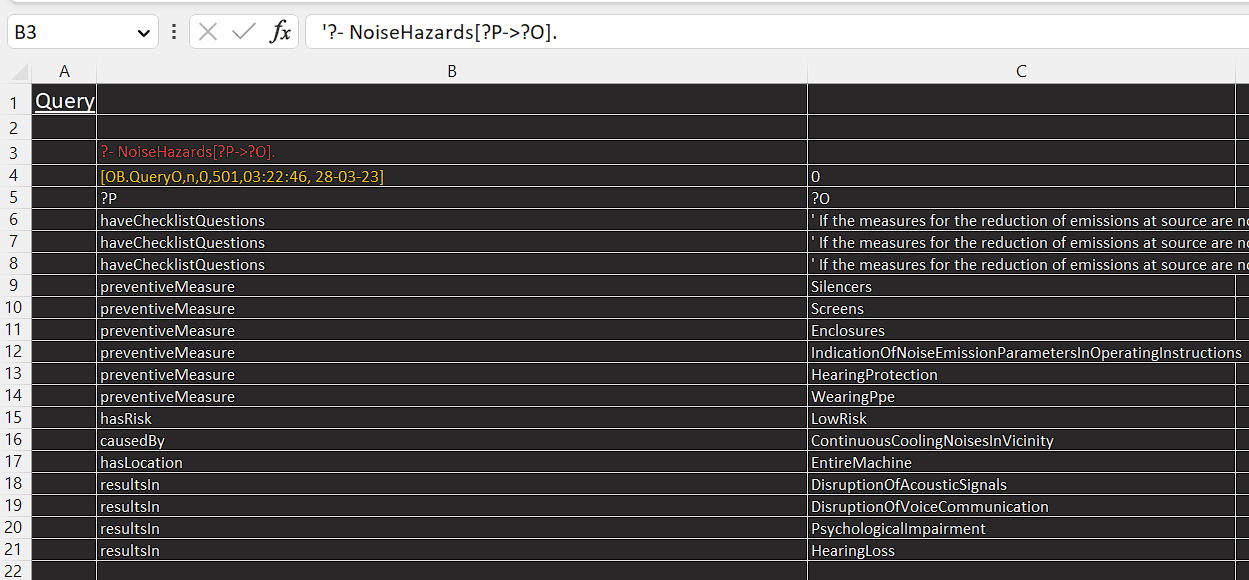
\includegraphics[width=\textwidth]{img/NoiseHazards.png}

\bigskip\bigskip \adjustimage{width=\textwidth, center, caption={Query on a hazard NoiseHazards from Laser}, label={fig18}, nofloat=figure, vspace=\bigskipamount}{img/NoiseHazards.png}

\begin{itemize}
    \item haveChecklistQuestions - This relation gives the checklist questions that need to be answered per hazard according to the ISO 12100. The safety standards mentioned as reference can be further queried to gain more information about them. For now, it only shows a brief title of the standard, but can further be expanded to allocate more data.
    \item preventiveMeasure - This relation gives the protection equipments and preventions required against the hazard. 
    \item hasRisk - Shows the risk rating of the hazard on a scale of high, medium or low.
    \item causedBy - This relation gives the possible reason of occurrence of the hazard.
    \item hasLocation - This relation gives the possible location of occurrence of the hazard on the machine.
    \item resultsIn - This relation gives the possible outcome of the hazard if it is not mitigated properly.
\end{itemize}

\bigskip\bigskip \adjustimage{width=\textwidth, center, caption={Graph visualisation of NoiseHazards from Laser}, label={fig18}, nofloat=figure, vspace=\bigskipamount}{img/noise_hazards_graph.png}

\paragraph{} All the above data could help the engineer to quickly have a glance at the important data required for the risk assessment. Also if required the engineer can update the knowledge graph with new hazard data if needed, and this information could be re-used in future risk assessment. Hence, the model could retain the expert's knowledge in a structured manner. At least that part of the expert's knowledge which can be easily formalised. 

\section{Specific use case} \label{specific_use}
In industrial risk assessment, Performance Level (PL) is an important concept particularly in the context of machinery safety. PL is used to determine the level of safety performance required of a safety-related control system or safety function, and is calculated based on the level of risk reduction required to ensure an acceptable level of safety. It is often calculated in 4 levels with level D being the being the highest level of safety performance. PL is typically used in the context of machinery safety and is based on the ISO 13849-1 standard, which provides guidelines for the design of safety-related control systems for machinery. % cite ISO 13849-1

\paragraph{} The importance of PL in industrial risk assessment lies in its ability to help ensure that machinery and equipment are designed and operated in a manner that minimizes the risk of harm to workers and the environment. By conducting a risk assessment and determining the PL required for a safety function or control system, designers and operators can implement appropriate measures to achieve the required level of safety performance. For example, if a risk assessment determines that a machine presents a high risk of injury to workers, a high PL may be required for the safety function or control system responsible for mitigating that risk. This may require the use of redundant safety features, such as emergency stop buttons, and the implementation of regular testing and maintenance procedures to ensure that the safety function or control system continues to perform at the required PL. 

\paragraph{} Now with the knowledge graph in place, finding the missing information regarding the performance level indicators is a simple task, that is, to just query the model. Hypothesis 3.1 can easily be tested here by querying all the information regarding performance level. On the other hand, hypothesis 3.2 which is about machine-to-machine communication of the performance level for automatic mitigation of risk, can be a topic of future research which can be built on top of this work. Hence Hypothesis 3.1 can be evaluated by the following query.

% \bigskip\bigskip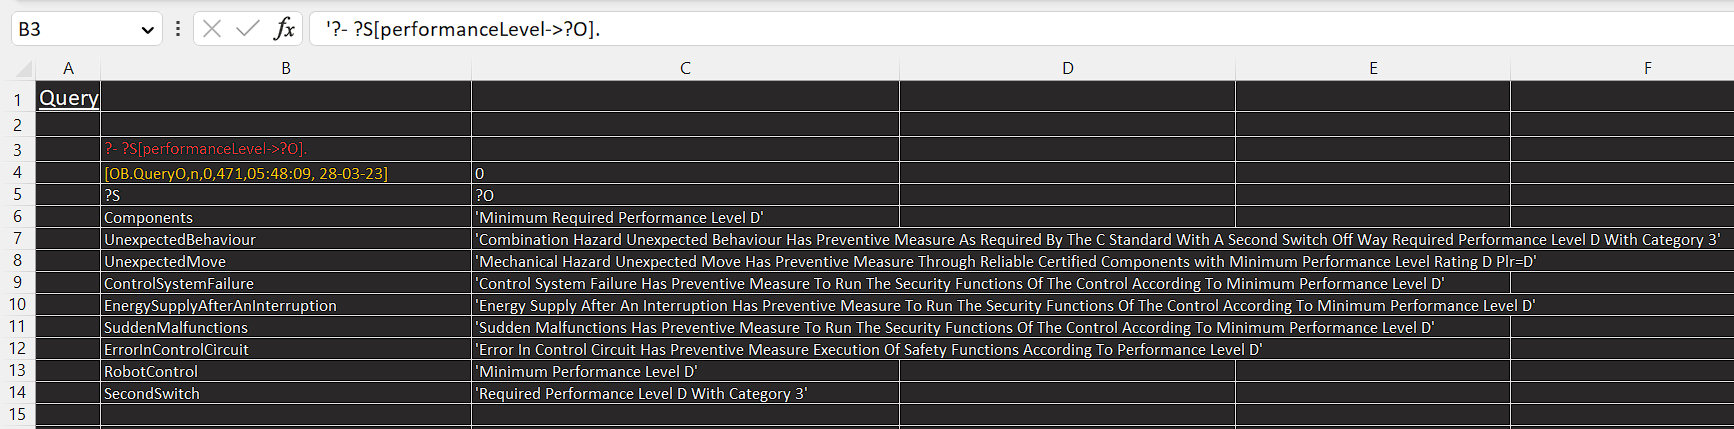
\includegraphics[width=\textwidth]{img/performanceLevel.png}

\bigskip\bigskip \adjustimage{width=\textwidth, center, caption={Query on the relation performanceLevel}, label={fig19}, nofloat=figure, vspace=\bigskipamount}{img/performanceLevel.png}

Another implementation of the knowledge graph for a very specific use case can be to search for the reference standards that are required for certain cases. This comes handy as the engineer don't need to search for the reference standard by reading through the whole document but can easily find the use cases where the reference standards are referred. A field search cannot work in this case because the reference standards are not always tagged with some keyword in the standard. Also further query on the reference standard gives a brief title of the standard which can further be expanded to accommodate the complete standard. The following query on reference standards can be cited as an example.

\bigskip \adjustimage{width=\textwidth, center, caption={Query on the relation referenceStandards}, label={fig20}, nofloat=figure, vspace=\bigskipamount}{img/referenceStandards.png}

\bigskip Alternately, if the engineer wants to find out about a particular standard 'EN ISO 13849-2' and in which cases it is referred to, the following query on the knowledge graph can suffice the purpose. This would be really helpful when the knowledge model have multiple standards. In that case searching manually for the use case of a particular reference standard would involve a lot of work.  

% \bigskip\bigskip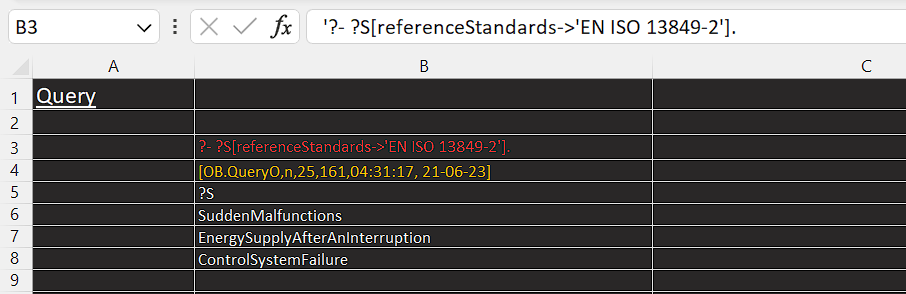
\includegraphics[width=\textwidth]{img/referenceStandards13849-2.png}

\bigskip \adjustimage{width=\textwidth, center, caption={Query on a particular reference standard}, label={fig20}, nofloat=figure, vspace=\bigskipamount}{img/referenceStandards13849-2.png}

